\documentclass[tikz,border=5]{standalone}
\renewcommand\familydefault\sfdefault
\usetikzlibrary{fit,shapes.geometric}
\pgfdeclarelayer{signal}
\pgfsetlayers{signal,main}
\tikzset{pics/.cd,
  SBS/.style={code={
      \begin{scope}[local bounding box=#1]
      \fill [pic actions/.try] (-1,0) -- (-1/2,3) -- (1/2, 3) -- (1,0) -- cycle;
      \fill [pic actions/.try] (-1/16,2) rectangle (1/16,4);
      \fill [pic actions/.try] (0,4) circle [radius=1/4];
      \foreach \i in {-1,1}
        \fill [shift=(90:4), xscale=\i]
          \foreach \r in {1,3/2,2}{
            (-45:\r) arc (-45:45:\r) -- (45:\r-1/10)
            arc(45:-45:\r-1/10) -- cycle
          };
       \end{scope}
  }},
  SU/.style={code={ 
    \begin{scope}[local bounding box=#1]
      \fill [even odd rule, pic actions/.try] 
        (-1,-5/2) -- (-1,-1/8) -- (1,-1/8) -- (1,-5/2)
        arc (360:180:1 and 1/4) -- cycle
     (-1,5/2) -- (-1,1/8) -- (1,1/8) -- (1,5/2)
        arc (0:180:1 and 1/4) -- cycle
     (-3/4, 9/4) -- (-3/4, 3/8) -- (3/4, 3/8) -- (3/4, 9/4) 
     arc (0:180:3/4 and 1/8)-- cycle
     \foreach \i in {-1,0,1}{\foreach \j in {1,2,3}{
       (-\i*1/2-3/16,-\j/2-3/4) rectangle ++(3/8, 3/8)}}
     (-1/2,-3/4) rectangle (1/2, -1/4);
   \end{scope}
  }},
  SIGNAL/.style={code={
    \begin{scope}[local bounding box=#1]
      \fill [pic actions/.try]
      (0,-3) -- (-1,1/2) -- (1/8,1/4) -- (0,3) -- (1,-1/2) -- (-1/8,-1/4)
      -- cycle;
    \end{scope}
  }}
}
\colorlet{sky blue}{blue!60!cyan!75!black}
\colorlet{dark blue}{blue!50!cyan}
\colorlet{chameleon}{olive!75!green}
\tikzset{signal/.style={draw=gray, line width=0.2em, dashed}}
\begin{document}
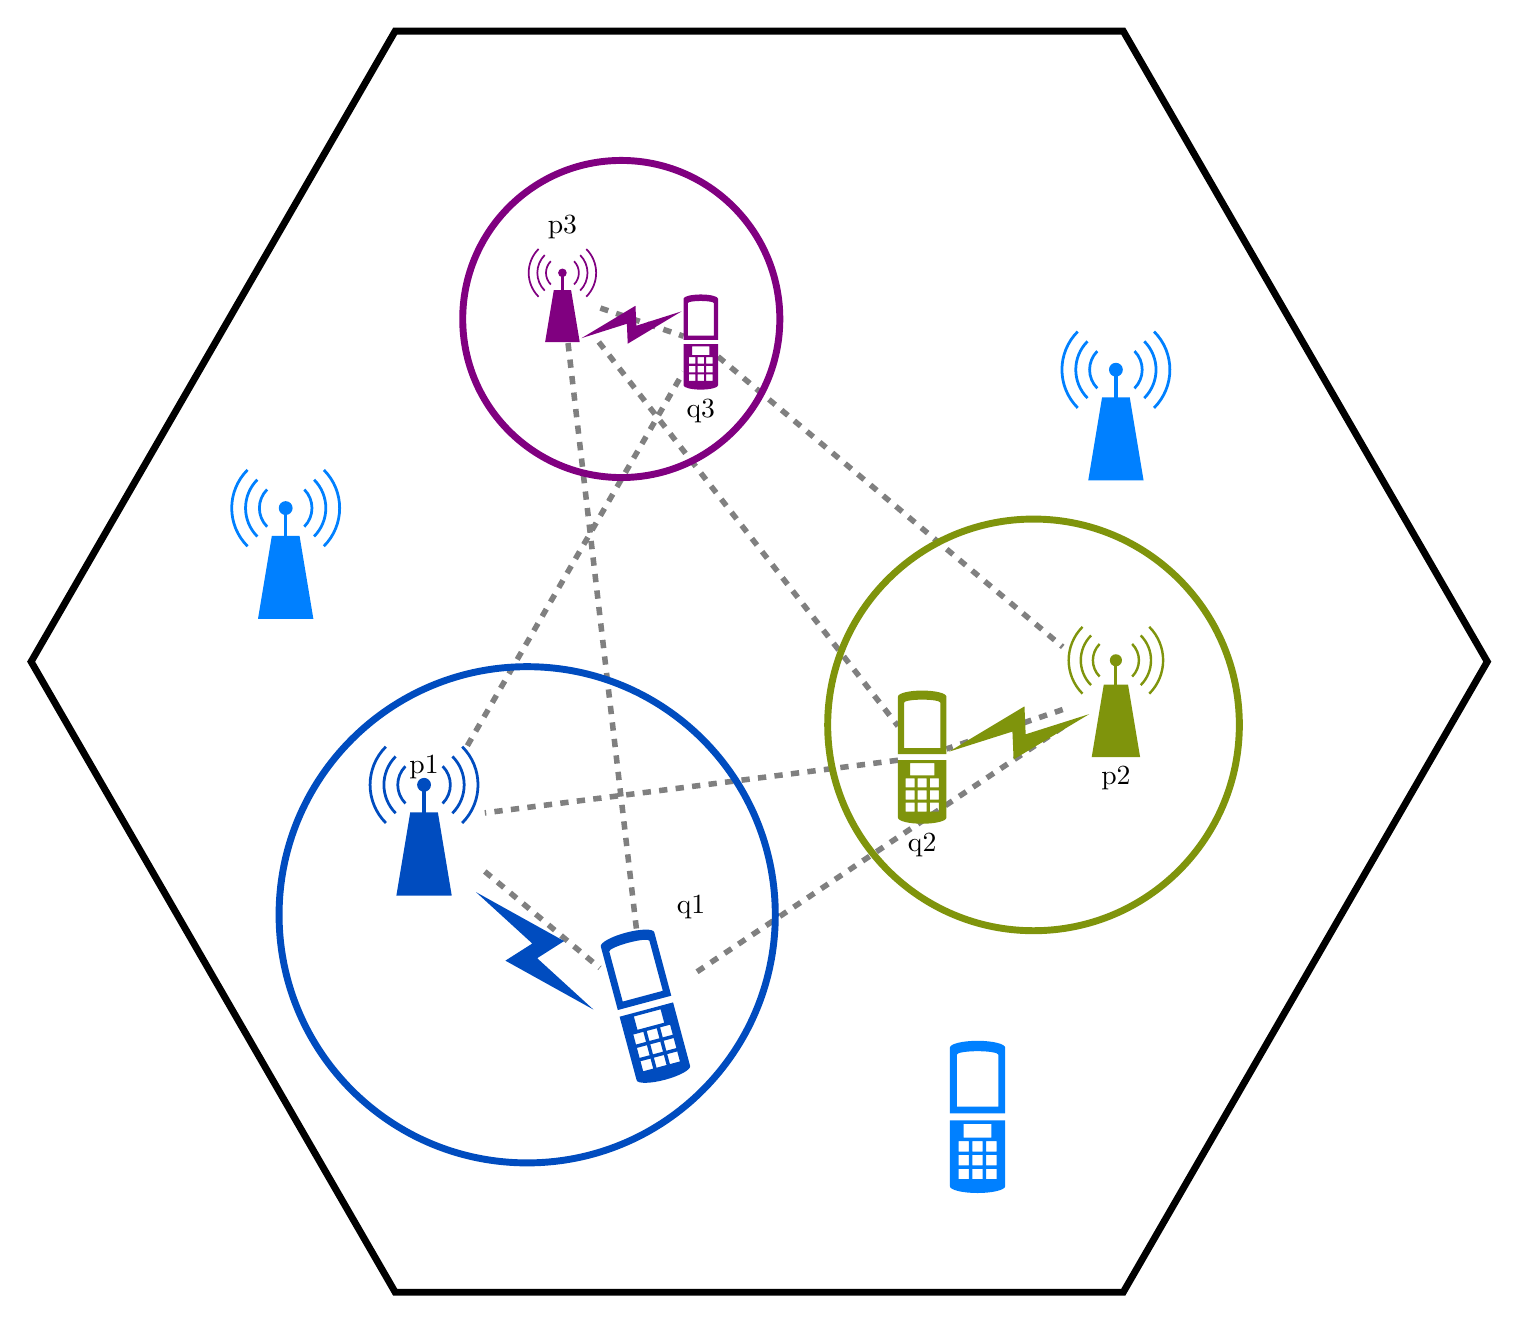
\begin{tikzpicture}[x=1em,y=1em]

\begin{scope}[local bounding box=b1]
\pic [fill=sky blue] {SBS=p1};
\pic [rotate=15, fill=sky blue]  at (8,-4)  {SU=q1};
\pic [rotate=45, fill=sky blue] at (4,-2)  {SIGNAL=s1};
\node [line width=0.25em,draw=sky blue, shape=circle, fit={(p1) (q1) (s1)}] {};
\path (p1.north) node [below] {p1} (q1.north east) node [above] {q1};
\end{scope}

\begin{scope}[shift={(25,5)}, x=1em*7/8, y=1em*7/8, local bounding box=b2]
\pic [fill=chameleon] {SBS=p2};
\pic [fill=chameleon]  at (-8,0)  {SU=q2};
\pic [rotate=-75, fill=chameleon] at (-4,1)  {SIGNAL=s2};
\node [line width=0.25em,draw=chameleon, inner sep=1em,
  shape=circle, fit={(p2) (q2) (s2)}] {};
\path (p2.south) node [below] {p2} (q2.south) node [below] {q2};
\end{scope}

\begin{scope}[shift={(5,20)}, x=1em*5/8, y=1em*5/8, local bounding box=b3]
\pic [fill=violet] {SBS=p3};
\pic [fill=violet]  at (8,0)  {SU=q3};
\pic [rotate=-75, fill=violet] at (4,1)  {SIGNAL=s3};
\node [line width=0.25em,  draw=violet, inner sep=1em,
  shape=circle, fit={(p3) (q3) (s3)}] {};
\path (p3.north) node [above] {p3} (q3.south) node [below] {q3};
\end{scope}

\begin{pgfonlayer}{signal}
\draw [signal] 
  (p1) -- (q3) -- (p2) -- (q1) -- (p3) -- (q2) -- (p1) 
  (p1) -- (q1) (p2) -- (q2) (p3) -- (q3);
\end{pgfonlayer}

\node [regular polygon, regular polygon sides=6, fit={(b1) (b2) (b3)},
draw=black, line width=0.25em, inner sep=-2em]
{};

\pic [fill=dark blue] at (-5, 10) {SBS};
\pic [fill=dark blue] at (25, 15) {SBS};
\pic [fill=dark blue] at (20, -8) {SU};
\end{tikzpicture}
\end{document}